% Options for packages loaded elsewhere
\PassOptionsToPackage{unicode}{hyperref}
\PassOptionsToPackage{hyphens}{url}
%
\documentclass[
]{article}
\usepackage{amsmath,amssymb}
\usepackage{lmodern}
\usepackage{iftex}
\ifPDFTeX
  \usepackage[T1]{fontenc}
  \usepackage[utf8]{inputenc}
  \usepackage{textcomp} % provide euro and other symbols
\else % if luatex or xetex
  \usepackage{unicode-math}
  \defaultfontfeatures{Scale=MatchLowercase}
  \defaultfontfeatures[\rmfamily]{Ligatures=TeX,Scale=1}
\fi
% Use upquote if available, for straight quotes in verbatim environments
\IfFileExists{upquote.sty}{\usepackage{upquote}}{}
\IfFileExists{microtype.sty}{% use microtype if available
  \usepackage[]{microtype}
  \UseMicrotypeSet[protrusion]{basicmath} % disable protrusion for tt fonts
}{}
\makeatletter
\@ifundefined{KOMAClassName}{% if non-KOMA class
  \IfFileExists{parskip.sty}{%
    \usepackage{parskip}
  }{% else
    \setlength{\parindent}{0pt}
    \setlength{\parskip}{6pt plus 2pt minus 1pt}}
}{% if KOMA class
  \KOMAoptions{parskip=half}}
\makeatother
\usepackage{xcolor}
\usepackage[margin=1in]{geometry}
\usepackage{graphicx}
\makeatletter
\def\maxwidth{\ifdim\Gin@nat@width>\linewidth\linewidth\else\Gin@nat@width\fi}
\def\maxheight{\ifdim\Gin@nat@height>\textheight\textheight\else\Gin@nat@height\fi}
\makeatother
% Scale images if necessary, so that they will not overflow the page
% margins by default, and it is still possible to overwrite the defaults
% using explicit options in \includegraphics[width, height, ...]{}
\setkeys{Gin}{width=\maxwidth,height=\maxheight,keepaspectratio}
% Set default figure placement to htbp
\makeatletter
\def\fps@figure{htbp}
\makeatother
\setlength{\emergencystretch}{3em} % prevent overfull lines
\providecommand{\tightlist}{%
  \setlength{\itemsep}{0pt}\setlength{\parskip}{0pt}}
\setcounter{secnumdepth}{-\maxdimen} % remove section numbering
\usepackage{booktabs}
\usepackage{longtable}
\usepackage{array}
\usepackage{multirow}
\usepackage{wrapfig}
\usepackage{float}
\usepackage{colortbl}
\usepackage{pdflscape}
\usepackage{tabu}
\usepackage{threeparttable}
\usepackage{threeparttablex}
\usepackage[normalem]{ulem}
\usepackage{makecell}
\usepackage{xcolor}
\ifLuaTeX
  \usepackage{selnolig}  % disable illegal ligatures
\fi
\IfFileExists{bookmark.sty}{\usepackage{bookmark}}{\usepackage{hyperref}}
\IfFileExists{xurl.sty}{\usepackage{xurl}}{} % add URL line breaks if available
\urlstyle{same} % disable monospaced font for URLs
\hypersetup{
  pdftitle={Predicting Credit Card Customer Total Transactions and If They Exit the Company},
  pdfauthor={Team 4: Henry Siegler, Jake Ketchner, Esteban Anderson},
  hidelinks,
  pdfcreator={LaTeX via pandoc}}

\title{Predicting Credit Card Customer Total Transactions and If They
Exit the Company}
\author{Team 4: Henry Siegler, Jake Ketchner, Esteban Anderson}
\date{}

\begin{document}
\maketitle

\hypertarget{introduction}{%
\subsection{Introduction}\label{introduction}}

This report is an investigation analyzing data on credit card customers
for a particular company to learn about the relationship between various
attributes of the credit card customers, such as their spending habits
and whether or not they are still current customers. The data was
obtained from kaggle
\href{https://www.kaggle.com/code/atillazkaymak/credit-card-customer-churn-prediction/data?select=BankChurners.csv}{at
this link}. The dataset is from an unknown credit card company and we
only are provided data for some of their customers that use of used to
use their credit card to some degree. We have 10,127 total observations.
Each observational unit in the study is a customer of the credit card
company, and the variables that we are focusing on are total transaction
amount in the past 12 months (in dollars), total transaction count in
the past 12 months, whether or not the customer is still with the
company (binary), total number of products held by the customer, and the
customer's credit limit (in dollars). For the simple and multiple linear
regression sections, we are considering total transaction count in the
past 12 months the response variable. For the logistic regression
section, whether or not the customer exited is the response variable,
which is a binary variable equal to 1 if the customer exited. Initially,
we hypothesize that total transaction amount and total transaction count
would be positively and linearly related, as it makes sense for
increased spending to be associated with an increased number of
transactions. We hypothesize that total transaction count to be
negatively correlated with if the customer exited, and positively
correlated with both credit limit and total number of products held by
the customer.

\hypertarget{descriptive-statistics}{%
\subsection{Descriptive Statistics}\label{descriptive-statistics}}

\textbf{Response Variable is Total Transaction Count}

In the table 1.1, we can see some descriptive statistics of the
variables in our dataset. None of the numeric variables have extremely
large maximum values relative to the average values for each of the
numeric variables.

Figure 1

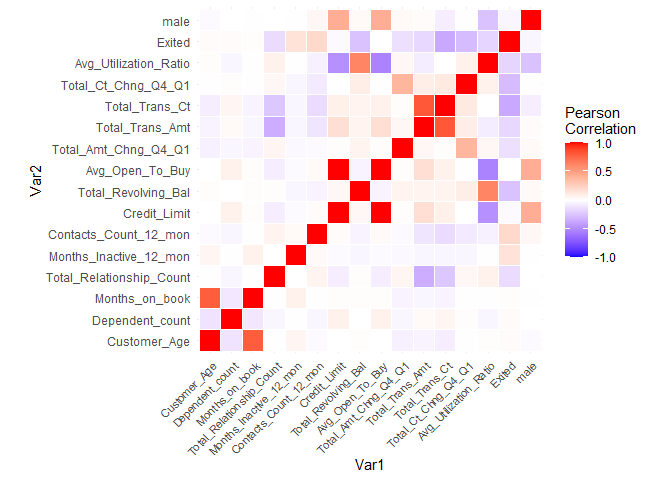
\includegraphics{Analysis_files/figure-latex/unnamed-chunk-5-1.pdf}

In Figure 1, we can see from the correlation matrix of the numeric
variables that \textbf{Avg\_Open\_To\_Buy} is highly correlated with
\textbf{Credit\_Limit}, so we will remove \textbf{Avg\_Open\_To\_Buy}
because it is redundant to keep both of these variables. We can see that
\textbf{Total\_Trans\_Ct} is highly correlated with
\textbf{Total\_Trans\_Amt}, which is what we would expect.
\textbf{Total\_Trans\_Ct}, the response variable, is moderately
negatively correlated with \textbf{Total\_Relationship\_Count}, which is
not what we would expect, because we would expect customers with more
products with the company to have more transactions. The response is
also moderately negatively correlated with \textbf{Exited}, which makes
sense because we would expect the customers who are not using the
company now to have less total transactions.

In table 1.3, looking at the actual correlations between the response
variable and all of the explanatory variables, we can see that the
variables with the highest correlation are \textbf{Total\_Trans\_Amt},
\textbf{Exited}, \textbf{Total\_Relationship\_Count}, and
\textbf{Contacts\_Count\_12\_mon}.

Now we will explore the \textbf{Total\_Trans\_Ct variable} and its
relationship with other correlated variables in our data.

Figure 2
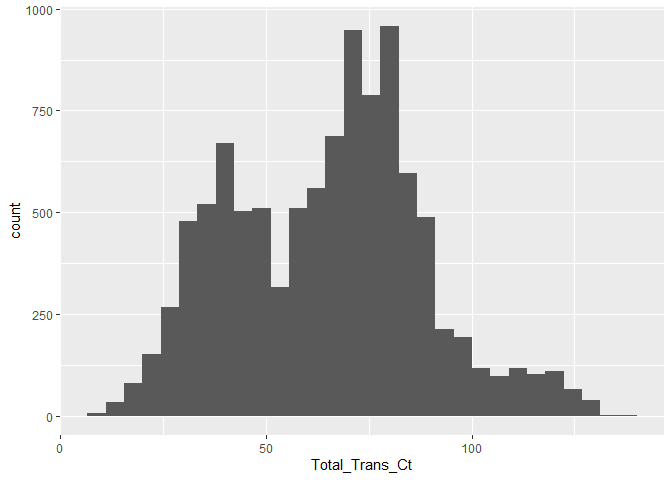
\includegraphics{Analysis_files/figure-latex/unnamed-chunk-7-1.pdf}

In figure 2, we see that most customers have a total transaction count
in the range of about 30 to 90 transactions in the past year.

Figure 3
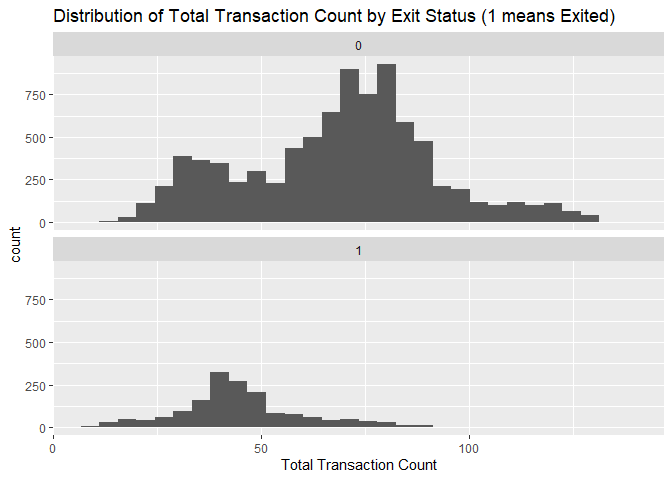
\includegraphics{Analysis_files/figure-latex/unnamed-chunk-8-1.pdf}

In figure 3, for all of the income categories, we see a bimodal
distribution for the \textbf{Total\_Trans\_Ct}. For people in the income
category of ``less than \$40K'', we see that there is a larger spike in
the second peak of the histogram compared to the other income
categories. However, looking at the general distribution of total
transaction count across the different income levels, the distributions
look pretty similar and have similar centers and averages, so it does
not appear that income category is related to the response.

Figure 4
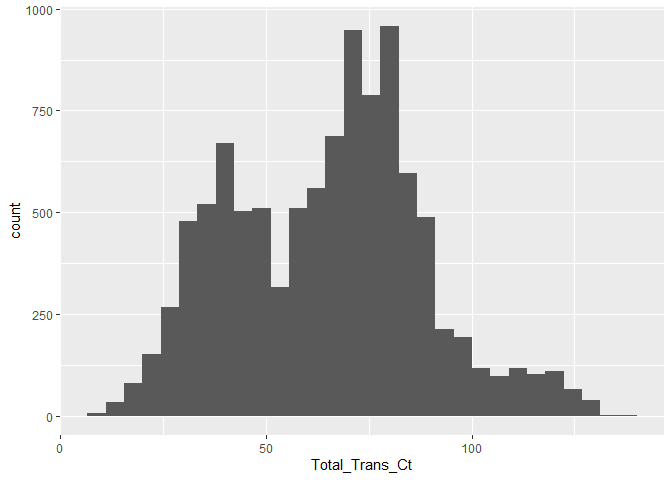
\includegraphics{Analysis_files/figure-latex/unnamed-chunk-9-1.pdf}

In figure 4, can see that the Total Transaction Counts for the customers
who have have exited has a unimodal distribution, with the center of the
peak being significantly below where most of the Transaction Counts are
for the customers who have not exited. The average total transaction
count for those who have exited appears to be about 35 transactions, but
that number is around 70 for those who have not exited. Therefore,
exited does appear to be very related to the response.

Figure 5
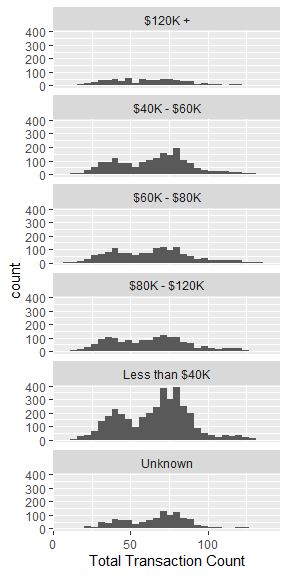
\includegraphics{Analysis_files/figure-latex/unnamed-chunk-10-1.pdf}

In Figure 5, we see that the average total transactions is smaller for
the groups of people with 3, 4, 5 and 6 products compared to those with
only 1 or 2 products. Total Relationship Count (total number of products
a customer has), appears to have a relationship with the response.

\hypertarget{data-visualization}{%
\subsection{Data Visualization}\label{data-visualization}}

Figure 6
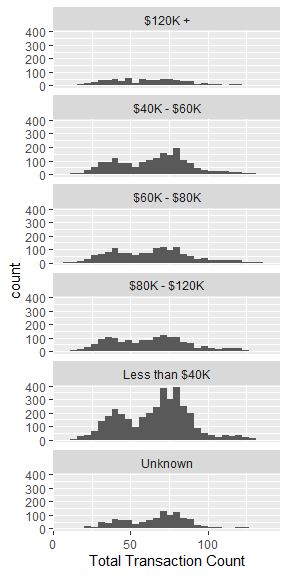
\includegraphics{Analysis_files/figure-latex/unnamed-chunk-11-1.pdf}

In Figure 6, based on the scatterplot between total transaction count
and total transaction amount, we can see that the data appears to form 3
clusters, and there are no customers who exited that were in the 3rd
cluster. Also, the data for both customers who exited and did not exit
appears to follow a 3rd degree polynomial relationship.

\hypertarget{data-cleaning}{%
\subsection{Data Cleaning}\label{data-cleaning}}

From our descriptive statistics earlier, we found that there were no
extremely large values for any of the variables, so we have no evidence
that any of the values in the dataset are incorrect entries.

Running a simple linear regression model predicting total transaction
count from total transaction amount, we see the following Cooks D
values:

Figure 7
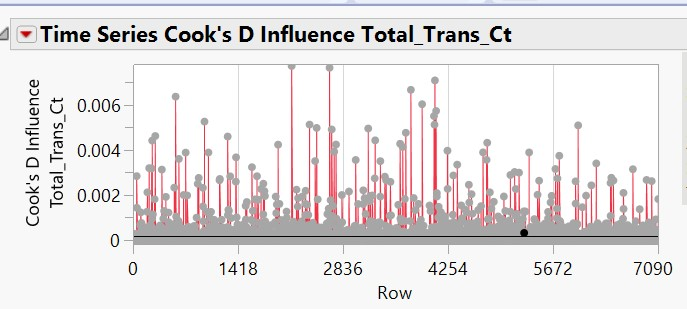
\includegraphics{https://github.com/hasiegler/STATProject/blob/main/SL12.jpg?raw=true}

In Figure 7, all of the Cook's D values are very low, because they are
much lower than 1. However, a few observations do stick out more than
others; 2 of the observations have values of about 0.008.

In Table 1.4, we can see that these two individuals have very high total
transaction amounts relative to the dataset as a whole. They have values
of \$16,563 and \$17,744, which are well above the 75th percentile, and
much closer to the maximum value of \$18,484. Their total transaction
counts are also very high: 94 and 104. These transaction counts are
higher than the 75th percentile for the data of 81. The very high values
for both the explanatory variable and the response for these individuals
explains why the Cook's D value is so high when a linear regression is
ran of these two variables. We do not have any reason to remove those
observations because their values are correct and they are not extremely
high.

\hypertarget{splitting-the-data}{%
\subsection{Splitting the Data}\label{splitting-the-data}}

We randomly selected 80\% of the observations and placed those into a
training dataset. The remaining 20\% of the data were placed into a
testing dataset.

\hypertarget{linear-regression}{%
\section{Linear Regression}\label{linear-regression}}

Explanatory Variable: \textbf{Total\_Trans\_Amt} Response Variable:
\textbf{Total\_Trans\_Ct}

Figure 8
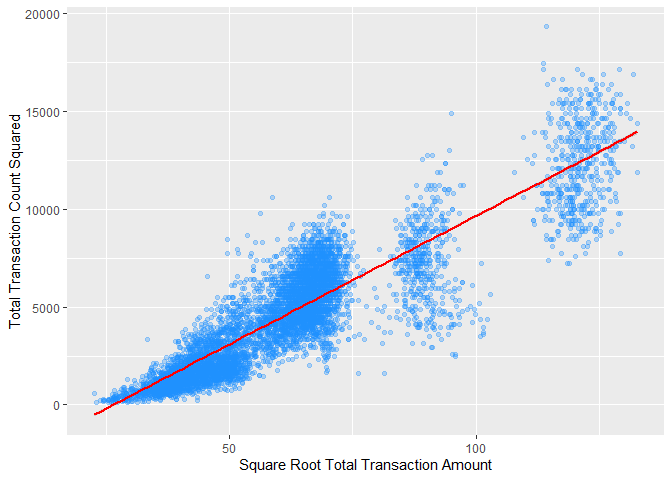
\includegraphics{Analysis_files/figure-latex/unnamed-chunk-13-1.pdf}

As we can see in the scatter plot in Figure 8, the relationship between
total transaction count and total transaction amount is not linear, so
we must apply transformations to make the relationship linear.

\hypertarget{variable-pre-processing}{%
\subsection{Variable Pre-Processing}\label{variable-pre-processing}}

\hypertarget{attempt-1}{%
\subsubsection{Attempt \#1}\label{attempt-1}}

First, we will try decreasing the power of the X variable, by taking the
square root. Also, we will increase the power of Y, by squaring the Y
variable.

Figure 9
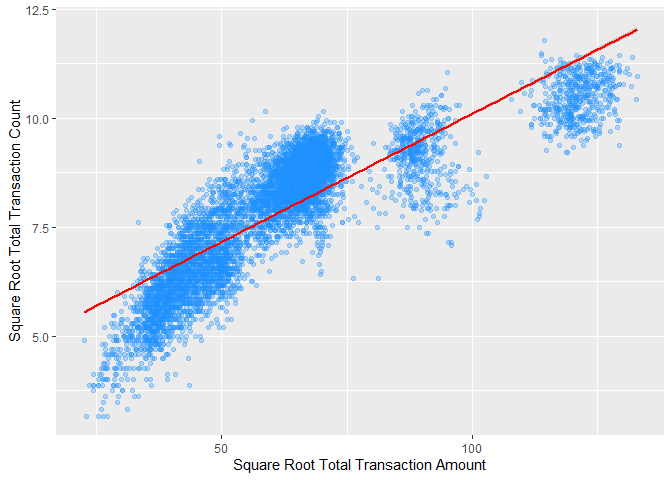
\includegraphics{Analysis_files/figure-latex/unnamed-chunk-14-1.pdf}

In Figure 9, linearity looks better, but equal error variance does not
appear to be satisfied. We have increasing variance, so we want to
decrease the power of Y to fix the unequal error variance. We will first
try the square root of Y instead of Y squared.

\hypertarget{attempt-2}{%
\subsubsection{Attempt \#2}\label{attempt-2}}

Figure 10
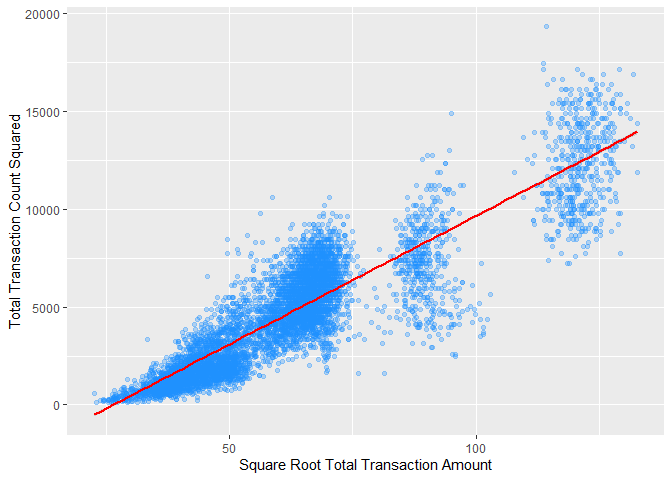
\includegraphics{Analysis_files/figure-latex/unnamed-chunk-15-1.pdf}

In Figure 10, equal error variance looks like it is satisfied, however
linearity does not look ideal. Therefore, we want to try to find a
transformation for Y that is between \(Y^{0.5}\) and \(Y^2\).

\hypertarget{attempt-3}{%
\subsubsection{Attempt \#3}\label{attempt-3}}

Figure 11
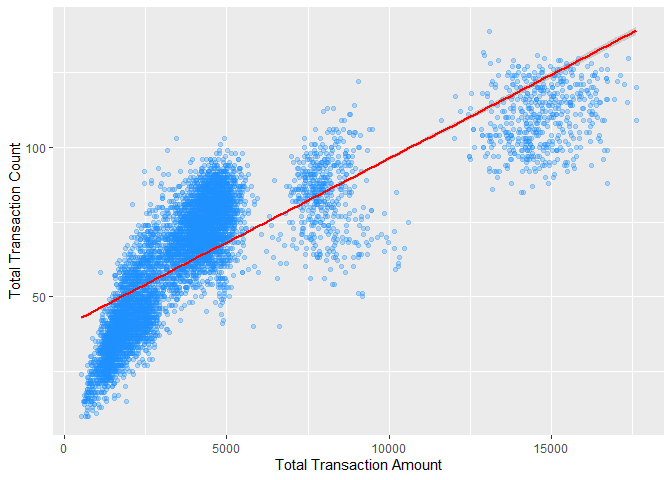
\includegraphics{Analysis_files/figure-latex/unnamed-chunk-16-1.pdf}

In Figure 11, raising total transaction count to the power of 0.8 keeps
the relationship fairly linear and maintains fairly equal error
variance. However, linearity does not look perfect, so let us continue
to decrease the power of X

\hypertarget{attempt-4}{%
\subsubsection{Attempt \#4}\label{attempt-4}}

Decreasing the power of X from 0.5 to 0.1, we get the following:

Figure 12
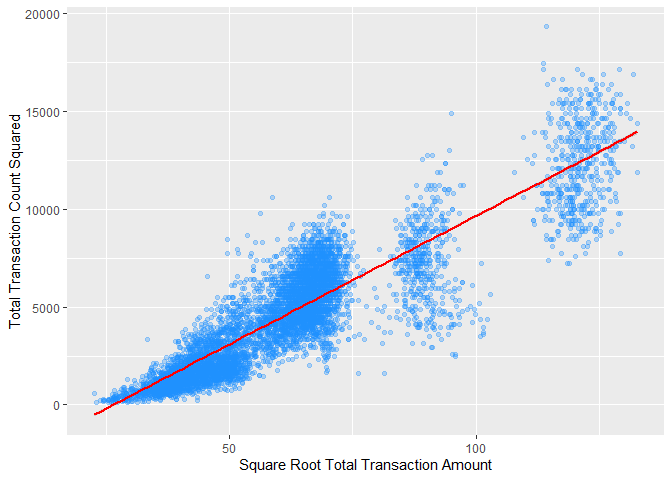
\includegraphics{Analysis_files/figure-latex/unnamed-chunk-17-1.pdf}

In Figure 12, these transformations seem to do the best job at
linearizing the data, while retaining equal error variances.

\hypertarget{residual-analysis}{%
\subsection{Residual Analysis}\label{residual-analysis}}

Therefore our current best transformations for simple linear regression
between \textbf{Total\_Trans\_Amt} and \textbf{Total\_Trans\_Ct} are:

X' = \(Total\_Trans\_Amt^{0.1}\) Y' = \(Total\_Trans\_Ct^{0.8}\)

\textbf{Equal Error Variance}

Figure 13
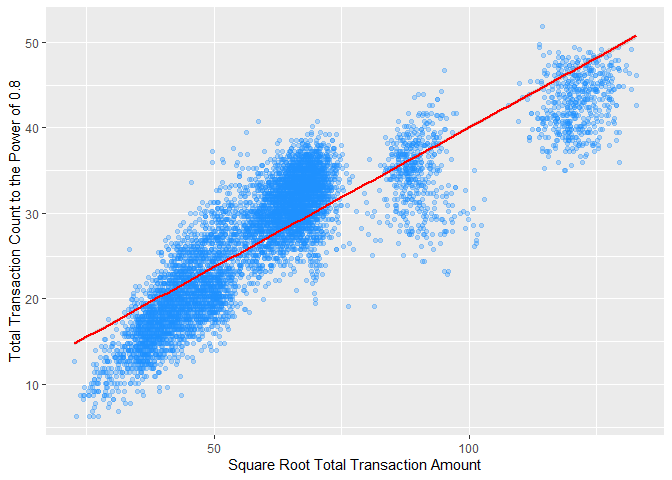
\includegraphics{Analysis_files/figure-latex/unnamed-chunk-19-1.pdf}

Based on the residual by predicted plot in Figure 13 and Brown-Forsythe
test in Table 1.5 with a small p value, we can conclude that equal error
variance is not satisfied. There residuals seem to fan out as the
predicted value increases.

\textbf{Linearity}

Linearity also does not look to be fully satisfied, with an F Ratio of
1.547 and a very small p value. Two of our assumptions are already
violated so we will try new transformations.

\hypertarget{new-transformation}{%
\subsubsection{New Transformation}\label{new-transformation}}

Figure 14
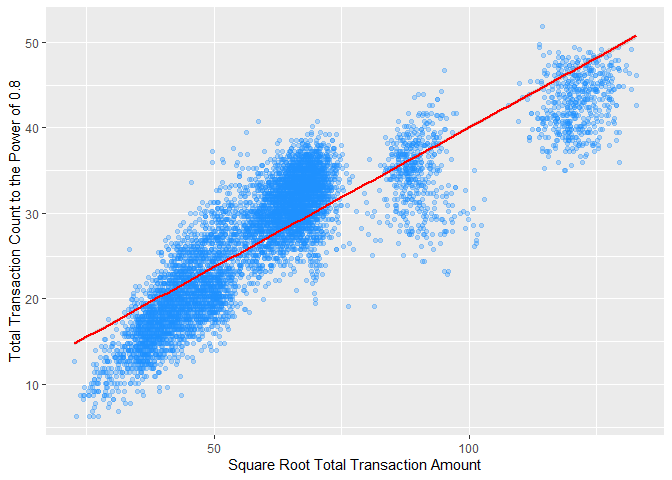
\includegraphics{Analysis_files/figure-latex/unnamed-chunk-20-1.pdf}

\textbf{Equal Error Variance}

Figure 15
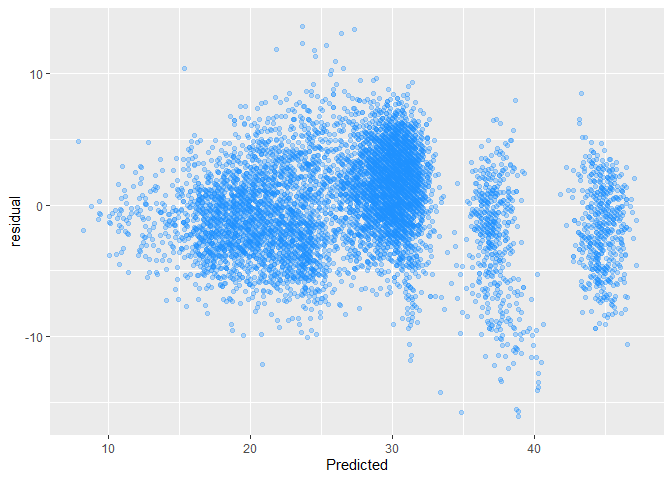
\includegraphics{Analysis_files/figure-latex/unnamed-chunk-22-1.pdf}

Looking at Figure 15 and Table 1.7, with this new transformation, we now
see that the equal error variance assumption is now satisfied based on
the large p value for the Brown-Forsythe test.

\textbf{Linearity}

We still cannot conclude that linearity is satisfied based on the lack
of fit test. However, the F ratio decreased to 1.34, which is an
improvement from 1.547 in the previous model. The F critical value for
these degrees of freedom is 1.057, so our F ratio is not too far above
this.

\textbf{Normality of Residuals}

Figure 16
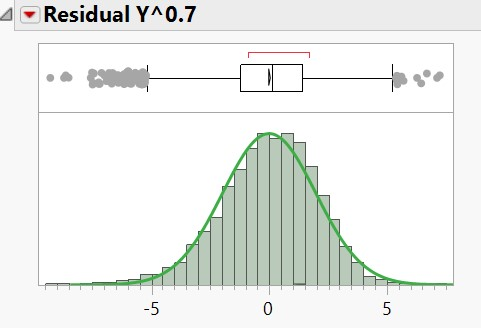
\includegraphics{https://github.com/hasiegler/STATProject/blob/main/SL6.jpg?raw=true}

Looking at Figure 16 and Table 1.9 we have a small pvalue for the
Anderson-Darling test, which indicates that we do not have normality of
residuals, the histogram of the residuals looks very normally
distributed, so we can conclude that this assumption is not terribly
violated.

\textbf{Independence}

Our data on the customers is sorted in a random order, so there is no
reason why the error of one observation would be related to the error of
the observation next to it. The Durbin-Watson value is 1.955, which is
very close to 2, which is the value that means there is no
autocorrelation. Our Durbin-Watson value has a pvalue of 0.03, which is
not significant at the alpha of 1\% level. Since we know that our data
is in a random order, and customers are likely not influencing each
other, we can conclude that independence is satisfied.

\hypertarget{unusual-observations}{%
\subsubsection{Unusual Observations}\label{unusual-observations}}

Figure 17
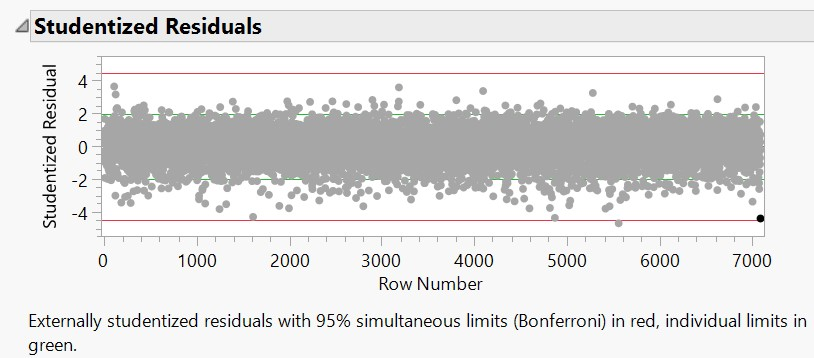
\includegraphics{https://github.com/hasiegler/STATProject/blob/main/SL8.jpg?raw=true}

In Figure 17, there are many externally studentized residuals greater
than 3 in absolute value. However, there is only 1 observation that is a
large outlier based on the Bonferroni adjustment.

Looking at Table 1.11 and Table 1.12, we can see that the customers with
the largest negative residuals almost all exited the company and had
high transaction amounts and lower transaction counts. For the customers
with the largest positive residuals, none of them have exited the
company, and they have much lower transaction amounts and high
transaction counts, relatively to other customers.

Figure 18
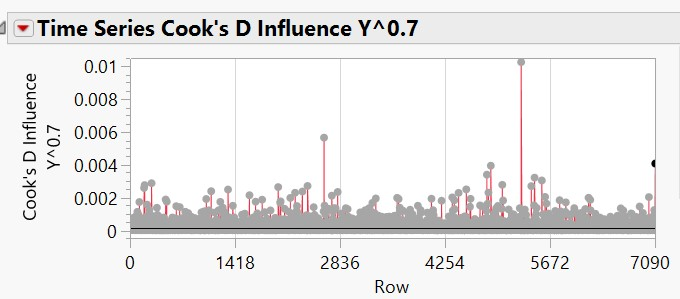
\includegraphics{https://github.com/hasiegler/STATProject/blob/main/SL9.jpg?raw=true}

In Figure 18, looking at the Cook's D Influence values, only a couple of
the observations stick out from the others. The Cook's D values are low,
since values of 0.5 or greater indicate that the observation is
influential. However, since one of the observations has a much higher
Cook's D value than the other points, that observation is likely
influential.

We view the attributes of this customer in Table 1.13. The customer has
a very low total transaction amount and a low total transaction count,
which may be the reason for why it has a Cook's D value so much greater
than the other observations.

\hypertarget{fit-a-linear-model}{%
\subsubsection{Fit a Linear Model}\label{fit-a-linear-model}}

Final Model:

\(X' = Total\_Trans\_Amt^{-0.2}\) \(Y' = Total\_Trans\_Ct^{0.7}\)

Figure 19
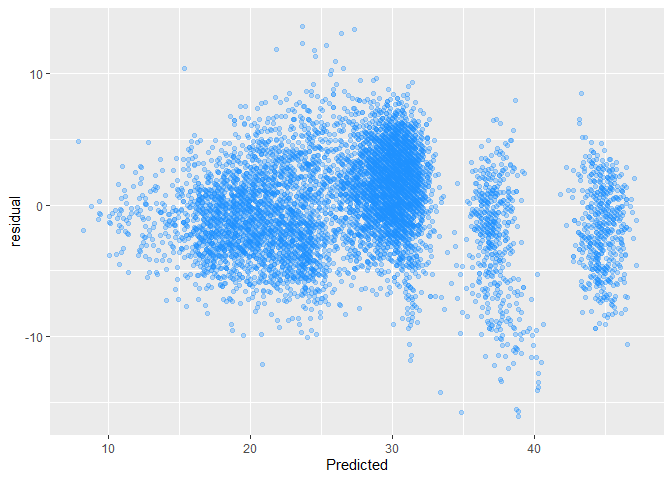
\includegraphics{Analysis_files/figure-latex/unnamed-chunk-23-1.pdf}

In Figure 19, the model not terribly violate any of the assumptions
required for simple linear regression models, so the predictions and
implications of our model should be fairly accurate and trustworthy. The
model does not account for omitted variable bias, which means that we
cannot interpret the slope coefficient as a causal effect of transaction
amount on transaction count.

From Table 1.14:

\(\widehat{Total\_Trans\_Ct}_i'=51.94 -170.88 Total\_Trans\_Amt_i'\)

The model does make sense contextually because the X variable was
transformed so that it was raised to the power of -0.2, so the negative
coefficient for the slope means that there is a positive relationship
between the untransformed variables. The variables have been transformed
greatly, so the coefficient estimates do not make sense to interpret.

Looking at Table 1.15, the model did a good job of explaining variation
in transaction count, as the R-squared value is 0.8281. Therefore,
82.8\% of the variation in the total transaction count transformed
variable is explained by the model. The root mean square error of the
model is 1.977, which is the typical deviation of the actual Y value
from the predicted Y value.

To interpret the intercept of the estimated regression equation, we can
say that the estimated total transaction count to the power of 0.7 is
51.9 when the total transaction amount is zero. This intercept does make
sense in context, however the minimum value of total transaction amount
in the data was \$510, so it may not be meaningful. For a 1 unit
increase in the tranaction amount to the power of -0.2, the transaction
count to the power of 0.7 decreases by 170.88.

\hypertarget{statistical-inference}{%
\subsection{Statistical Inference}\label{statistical-inference}}

\(H_0\): The model is not significant. \(H_A\): The model is
significant.

In Table 1.16, the F ratio for the test of overall model significance is
34,217, which is very large, meaning that we can conclude that our model
is significant.

\hypertarget{confidence-interval-and-prediction-interval}{%
\subsubsection{Confidence Interval and Prediction
Interval}\label{confidence-interval-and-prediction-interval}}

We are interested in calculating confidence intervals for the mean of
individuals with transaction amounts of \$6000, because there is a large
cluster of customers who spent about that much total.

From Table 1.17 customers with transaction amounts of \$6000, we are
95\% confident that the true mean transaction count to the power of 0.7
is between 21.88 and 22.004.

For a single new customer with a transaction amount of \$6000, we are
95\% confident that that customer's actual transaction count to the
power of 0.7 is between 18.06 and 25.82.

\hypertarget{model-validation}{%
\subsection{Model Validation}\label{model-validation}}

Using the linear regression model that was built using the training
data, we calculate the predicted values for all the observations in the
testing data. The correlation between those predicted values and the
actual response values for the testing data is 0.9109, which is a very
high correlation, meaning that our model still did a good job at
predicting out of sample values.

\hypertarget{conclusion}{%
\subsection{Conclusion}\label{conclusion}}

In order to investigate the relationship between transaciton amount and
transaction count over the past 12 months for all of the customers of
the credit card company in the dataset, we first had to transform our
variables so that the assumptions for simple linear regression were met.
Linearity and equal error variance were clearly not met before we
applied transformations to the variables. After transforming the
variables, equal error variance was satisfied, linearity was very close
to being satisfied even although the lack fit test was not passed, and
normality of errors looked satisfied. The final transformed model did a
very good job in explaining variation in the response, with an R squared
value of 0.8281. The model utility test demonstrated that our model is
very significant, and we see that we have very statistically
significants for the coefficient estimates for the intercept and the
explanatory variable. There were not any extremely large residuals in
our model, and there was only a couple of observations that could have
been influential.

In terms of finding the best transformations, many different
combinations of transformations were attemped, and none of them seemed
to fully remedy the linearity assumption, however the data does seem to
have a linear form, so any conclusions made from the model should be
close to accurate, as no assumptions were highly violated. We would have
liked to have found a model that satisfied the lack of fit test, however
we reduced the F ratio for this test to be not too high, which we felt
was the best we could have done. We expected a positive correlation
between these two variables, which is what we discovered. We found that
the largest residuals in absolute value in our model were negative
residuals, meaning that the model over predicted the response for these
observations. We found it interesting that almost all of the
observations with the largest negative residuals were individuals that
had exited the credit card company. We found it interesting that one of
the observations had a much higher Cook's D value than the others, but
this customer had the minimum total transaction amount at \$510.

One thing that we were not fully content with in our analysis is that
the customers that we received information on were not all of the
customers of the credit card company. The minimum value of the total
transaction amount variable in the dataset was \$510, so these customers
all used their cards a reasonable amount. Also, there were no customers
with extremely large values for any of the variables, such as
transaction amount or credit limit, so it would have been nicer to know
more about how this data was collected.

\hypertarget{multiple-regression}{%
\section{Multiple Regression}\label{multiple-regression}}

\textbf{Response Variable: Total Transaction Count} \textbf{Explanatory
Variables: Total transaction amount, Exited (qualitative), Total
relationship count, Credit Limit}

\hypertarget{data-visualization-1}{%
\subsection{Data Visualization}\label{data-visualization-1}}

Figure 20
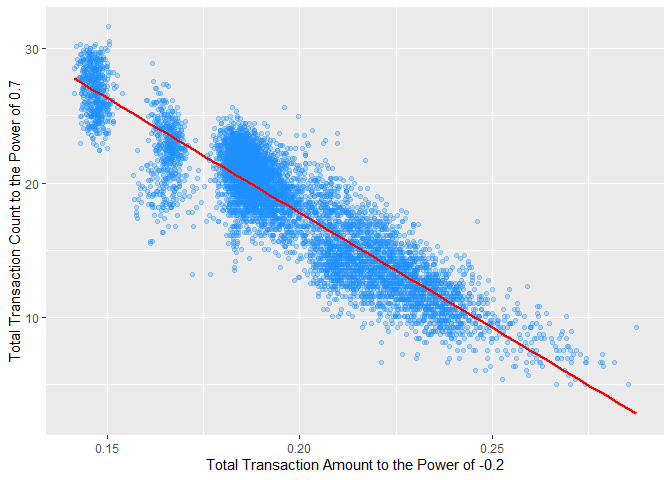
\includegraphics{Analysis_files/figure-latex/unnamed-chunk-24-1.pdf}

Figure 21
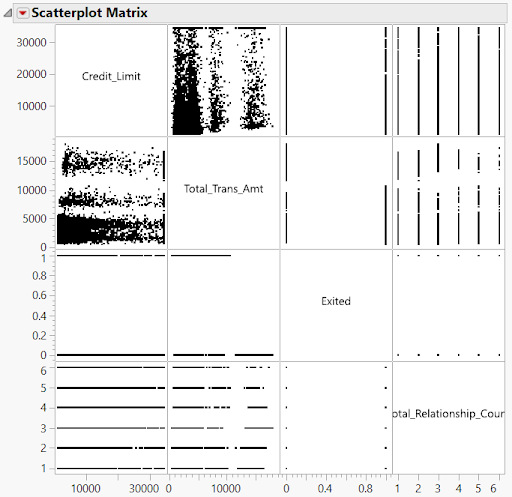
\includegraphics{https://github.com/hasiegler/STATProject/blob/main/ML1.png?raw=true}

Looking at Figure 20 and Figure 20, we can see explanatory variable that
seems most strongly associated with transaction count is total
transaction amount with a correlation of 0.807. In Table 1.19, we have
the values of the correlations, and exit status also seems moderately
correlated with the response, with a correlation of -0.37. We know that
total transaction count and total transaction amount do not have a
completely linear relationship, from our investigation in the simple
linear regression section. Exit status is a binary variable so we are
not worried about having a linear relationship with that variable and
the response. None of the explanatory variables are highly correlated
with each other, although total transaction amount and total
relationship count do have a correlation of -0.35, but that is not
extremely high. All of the variables behaved as we would had expected,
since increased transactions in amount and by count are positively
correlated with credit limit, and negatively correlated with exit
status. However, we found it unusual that total relationship count (the
number of products held by the customer), is negatively correlated with
transaction count and amount.

Figure 22
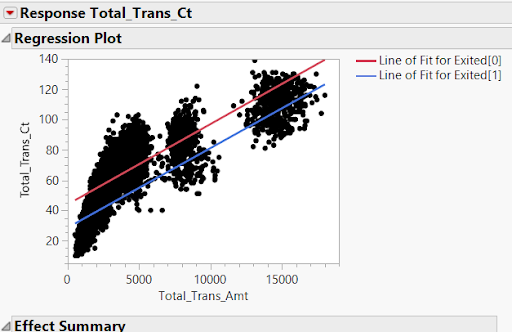
\includegraphics{https://github.com/hasiegler/STATProject/blob/main/ML2.png?raw=true}

Based on the graph in Figure 22 of with the interaction between Exit and
total transaction amount, we can see that there is almost no interaction
between these variables because the slopes of the lines look almost
perfectly parallel. The interaction term in the model allows the slope
between the X and Y variables to be different for customers who exited
and did not exit, and since the slopes look parallel we would expect the
interaction term to not be significant.

\hypertarget{variable-pre-processing-1}{%
\subsection{Variable Pre-Processing}\label{variable-pre-processing-1}}

Initial residual vs predicted plot with all of the untransformed
variables:

Figure 23
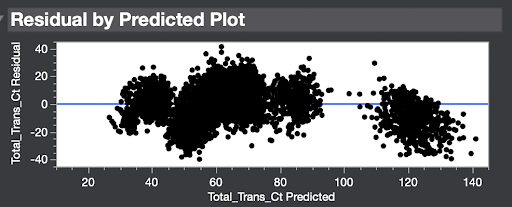
\includegraphics{https://github.com/hasiegler/STATProject/blob/main/ML3.png?raw=true}

Figure 24
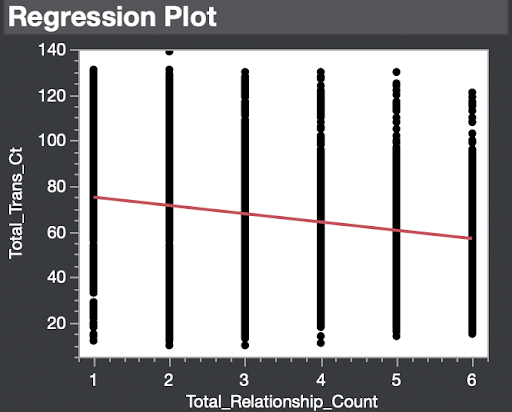
\includegraphics{https://github.com/hasiegler/STATProject/blob/main/ML4.png?raw=true}

In Table 2.1 original plot of total transaction count vs Total
relationship amount had linearity issues with a high F ratio of 61.46 in
the Lack of Fit Test, and a small p value of \textless0.0001.

After transforming the data by raising total relationship count to the
power of 0.5 we were able to attain a more linear model. In Table 2.2,
although it does not satisfy the lack of fit test, it is an improvement.
If we wanted to satisfy the lack of fit test we would most likely have
to transform the Y variable which would increase the complexity of our
model and force us to transform the other X variables as well.

From the analysis in the simple linear regression portion, we know that
total transaction count and total transaction amount do not have a
linear relationship. Therefore, we will raise total transaction amount
to the power of 0.001 and assess the linearity.

Figure 25
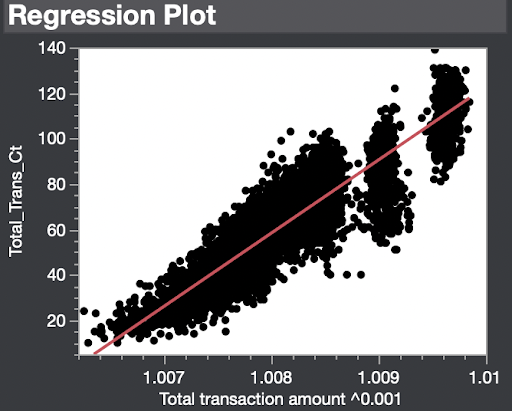
\includegraphics{https://github.com/hasiegler/STATProject/blob/main/ML7.png?raw=true}

After transforming total transaction amount by raising it to the power
of 0.001, we were able to attain a more linear model. In Table 2.3,
although it does not satisfy the lack of fit test, it is a large
improvement from the untransformed variables. If we wanted to satisfy
the lack of fit test we would most likely have to transform the Y
variable which would increase the complexity of our model and force us
to transform the other X variables as well.

Our final model is:

\textbf{Response Variable: Total Transaction Count} \textbf{Explanatory
Variables: Total transaction Amount to the power of 0.001, Exited
(qualitative), Total relationship count to the power of 0.5, Credit
Limit}

\hypertarget{residual-analysis-1}{%
\subsection{Residual Analysis}\label{residual-analysis-1}}

Now we will check the assumptions of our model.

\textbf{Linearity}

Figure 26
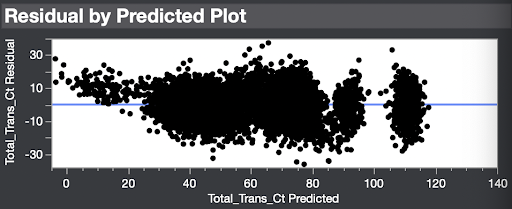
\includegraphics{https://github.com/hasiegler/STATProject/blob/main/ML9.png?raw=true}

Looking at the predicted values versus residual plot in Figure 26, we
can see that the say that linearity is met, as well as equal error
variance, as there is no fanning pattern in the data and the residual
line of zero goes through the middle of the data generally.

In Table 2.4, the lack of fit test also suggested that linearity is
satisfied, as the p value is 0.568 resulting in accepting the null
hypothesis that linearity is satisfied.

\textbf{Independence of Errors}

From Table 2.5, we can say that the independence of errors assumption is
satisfied because each of the customers in the dataset are likely
independent of each other and are not influencing each other in terms of
their transactions and the other variables in the model. The dataset is
also sorted in a random order with no time series component. Also, with
a Durbin-Watson value of 1.97, we can conclude there is no
autocorrelation.

Figure 27
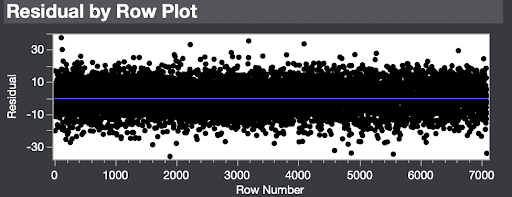
\includegraphics{https://github.com/hasiegler/STATProject/blob/main/ML12.png?raw=true}

We also look at the residual vs row order plot in Figure 27, which shows
no pattern, so we can conclude independence.

\textbf{Normality of Residuals}

Figure 28
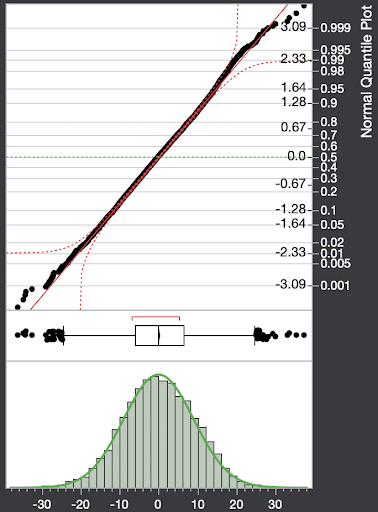
\includegraphics{https://github.com/hasiegler/STATProject/blob/main/ML13.png?raw=true}

Despite a low p-value for the Anderson-Darling test, which indicates
that the residuals are not normal, the histogram of the residuals
appears very normally distributed, so we can conclude that the normality
of residuals assumption is satisfied for this analysis.

Based on all of the tests to check the assumptions, none of the
assumptions are highly violated, so we can conclude that all of the
assumptions of multiple linearity regression are met, so we can move
forward with the model without worrying about inaccurate results. Our
sample size is so large that perfectly satisfying all of the tests is
not fully necessary, as long as the assumptions look generally
satisfied.

\hypertarget{fit-a-multiple-linear-regression-model}{%
\subsection{Fit a Multiple Linear Regression
Model}\label{fit-a-multiple-linear-regression-model}}

\(\widehat{Total\_Trans\_Ct} = -30,982 + 30,786Total\_Trans\_Amt^{0.001} - 0.55Total\_Relationship\_Count^{0.5} + 11.3Exited[0] - 0.00007Credit\_Limit\)

Looking at Table 2.7, certain aspects of our model do not make much
sense contextually. For example, an intercept of -30,982 does not make
sense in context, because that is a negative transaction count. However,
there are no observations in the dataset with any values for total
transaction count close to 0, which is why the intercept is negative.
Therefore, extrapolating predictions from this model would provide us
with invalid predictions. By transforming two of the variables we expect
a more difficult interpretation of the model's parameter estimates. The
initial model without transformations had an intercept of 38.025 and a
total transaction amount slope of 0.0053 which make more sense in
context of the problem. Our current model shows the relationship between
the response variable, total transaction count, and the four explanatory
variables; exited, total relationship count, credit limit, and total
transaction amount after they have been transformed.

Looking at Table 2.8, our model does a very good good of explaining
variation in the total transaction count. There is an R squared adjusted
value of 0.852. This means that 85.2\% of the variation in total
transaction count is explained by the explanatory variables in the
model, after accounting for the number of predictor variables in the
model.The error of our model or, root mean square error, is 8.99 that
the average absolute value of the error of our model in predicting total
transaction count is 8.99.

The interpretation of the intercept is that the average predicted total
number of transactions is -30,982 for an individual that does not spend
any amount, has 0 products with the company, has exited the company, and
has a credit limit of 0. The coefficient of the exited variable can be
interpreted as when the other variables constant, customers who have not
exited make 11.3 more transactions on average compared to customers who
have exited. We can also interpret the coefficient estimate of the
credit limit. With an increase of \$1000 in a customer's credit limit,
the predicted transaction count decreases by 0.07 on average, holding
all of the other variables constant.

To check the model for multicollinearity, we will analyze the variance
inflation factors (VIF) for each of the explanatory variables in Table
2.9. A maximum VIF value greater than 10 indicates that
multicollinearity is influencing the least squares estimate. The largest
VIF is on the total relationship count variable, with a value of 1.17,
which is not high at all and very close to 1. It says that the variance
of the estimated slope of total relationship count is increased 1.17
times due to the correlation with the other variables in the model.
Since all the VIF values are low, we can conclude that multicollinearity
is not influencing our model.

\hypertarget{statistical-inference-1}{%
\subsection{Statistical Inference}\label{statistical-inference-1}}

\textbf{Model Utility Test}

Ho: All of the coefficients in the model are equal to 0 or the model is
not significant Ha: At least one of the coefficients in the model does
not equal 0 or the model is significant

In Table 2.10 a p value of \textless0.0001 for the model utility test,
we reject the null hypothesis and conclude that our model is
significant.

\textbf{F Partial Test}

We will compare our model to a model with only one explanatory variable:
Total transaction amount to the power of 0.001, which is a variable in
the full model.

Ho: All of the coefficients in the full model not in the reduced model
are equal to 0 Ha: At least one of the coefficients in the full model
not in the reduced model is not equal to 0

F = {[} (691,464 - 573,585) / (7087 - 7084) {]} / 81 = 485.09

The F value for the F partial test is 485 with an associated p value
value of \textless0.0001, so we conclude that at least one coefficient
removed from the full model does not equal zero and therefore our full
model is significantly better than the reduced model with only total
transaction amount to the pwoer of 0.001.

\textbf{Interaction Analysis}

In the graph for the interaction between Exit and total transaction
amount with the response variable being transaction count, we will
investigate whether or not the interaction term is significant.

Ho: The relationship between total transaction amount and total
transaction count does not change depending on if a customer has exited
or not. Ha: The relationship between total transaction amount and total
transaction count changes depending on if a customer has exited or not.

In Table 2.11, the t test for the test of significance of the
interaction term has one degree of freedom and t ratio of 0.32. The
associated p value is 0.75, so we can conclude that the relationship
between total transaction amount and total transaction count does not
change depending on if a customer has exited or not. This matches the
graph from above, because the lines for the customers that exited and
did not exit look almost perfectly parrellel, suggesting that there is
no interaction.

\textbf{Confidence and Prediction Intervals}

We would like to predict a confidence interval for the mean transaction
counts and a prediction interval for the transaction counts for a given
customer. In Table 2.12, for a customers that have a transaction amount
of \$6,0000, a credit limit of \$11,000, four total products, and did
not Exit, we are 95\% confident that the mean total transaction count is
between 82.78 and 83.38 transactions. For a single customer with these
same combination of attributes, we are 95\% confident that the
customer's total transaction count will be between 65.42 and 100.74
transactions, which is a much larger range than the confidence interval.
This choice of explanatory variables is of interest because there are
many customers with this combination of attributes, and we would like to
see the intervals for customers who spend more than most customers,
which is why we choose a transaction count of \$6,000.

\textbf{Possible Extra: Richer Model and Interpretation}

Figure 29
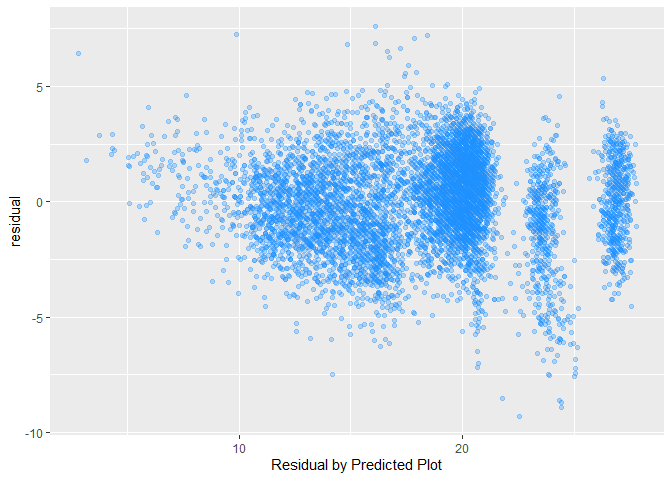
\includegraphics{Analysis_files/figure-latex/unnamed-chunk-26-1.pdf}

Based on the shape of the data in the scatterplot in Figure 29 between
total transaction amount and total transaction count, we can see that a
third degree polynomial explains the shape of the data well.

We will add the squares and cubed transaction amount terms to the model,
as well as a categorical variable for marital status, which has four
different categories: divorced, single, married, and unknown. We will
one-hot encode these variables and we will use marital status of single
as the baseline. We will also include total relationship count and exit
status into the model.

Figure 30
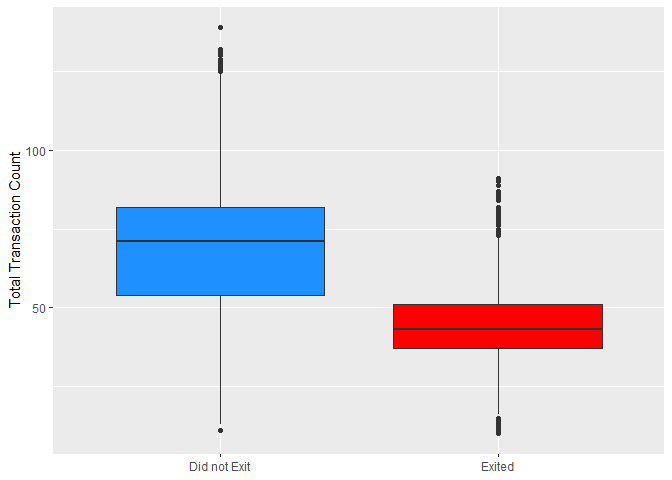
\includegraphics{Analysis_files/figure-latex/unnamed-chunk-29-1.pdf}
Looking at the predicted vs residual plot for the richer model in Figure
30, we can see that linearity and equal error variance are reasonably
satisfied.

When we look at the coefficient estimates in the model in Table 2.13, we
can see that the coefficients on the squared and cubed terms for
transaction amount are both significant, which suggests that a cubic
term for this variable is appropriate for explaining the data. We also
have significant coefficient estimates for married and unknown marital
status, meaning that when holding the other variables constant, there is
a significant difference in transaction counts between single customers
and married customers, and single customers and customers with an
unknown marital status. In particular, married and customers of unknown
marital status make about one fewer transaction than single customers,
holding the other variables constant. The coefficient for the divorced
estimate is not significant, meaning that predicted transaction count is
not different between single and divorced customers, holding all of the
other variables constant.

The adjusted R-squared value for this model is 0.855, which is only
slightly higher than the adjusted R-squared value in our original
multiple linear regression model of 0.852.

\hypertarget{model-validation-1}{%
\subsection{Model Validation}\label{model-validation-1}}

Using the original multiple linear regression model without the
polynomial terms for transaction amount, we will predict values for the
testing data using the model from the training data and evaluate the
results.

Using the coefficients of the model created using the training data, we
predicted all of the values for the testing data. The correlation
between those predicted values and the actual transaction counts for the
testing data customers is 0.92 from Table 2.14, which is a high
correlation, suggesting that our model does a good job of predicting
values out of sample. Also in Table 2.15, the root mean square error
found from the testing data actual values and their predicted values is
9.05, which is only slightly higher than the root mean square error of
the training model, which was 8.99. This also suggests that our model
has not been overfit to the training data because it is still very good
at predicting values for customers that were not in the dataset used to
create the model.

\hypertarget{conclusion-1}{%
\subsection{Conclusion}\label{conclusion-1}}

Overall, the final model is very strong and it predicts the total
transaction count of customers fairly accurately, with a typical
deviation of actual values from predicted values of 9, which is very
close considering the average transaction count is 65 transactions. The
model is not overfit to the training data, as it does just about as good
at predicting values out of sample in the testing dataset as it does
predicting values in the training dataset. The overall model utility
test suggests that our model is very significant in predicting
transaction count for these customers of this company.

The model is valid, as it generally satisfies all of the assumptions
required for multiple linear regression models. One weakness of the
model is that it is only a slight improvement in predicting transaction
count compared to the simple linear regression model with only
transaction amount transformed as a predictor variable. The R squared
values for both of these models are similar, and our model is more
complex due to the extra terms that were added to the model.

The final does tell us a few things about the total transaction counts
for customers. It tells us customers that have not exited generally have
more transactions compared to customers that exited, so if a customer is
not engaging in as many transactions, they are more likely to exit.
Also, as the total number of products held by a customer increases, the
less transactions the customer has on average, holding the other
variables constant. Also, we can see that increased transaction amounts
are associated with higher transaction counts, holding the other
variables constant.

It would be beneficial to one hot encode all of the categorical
variables in the dataset, such as income level and education status, and
compare how the different education or income levels relate to the
transaction counts when holding other variables constant.

\hypertarget{logistic-regression}{%
\section{Logistic Regression}\label{logistic-regression}}

\hypertarget{descriptive-statistics-1}{%
\subsection{Descriptive Statistics}\label{descriptive-statistics-1}}

\textbf{Binary Response Variable: Exited (1 Meaning the Customer Exited
or Left the Company)}

Figure 31
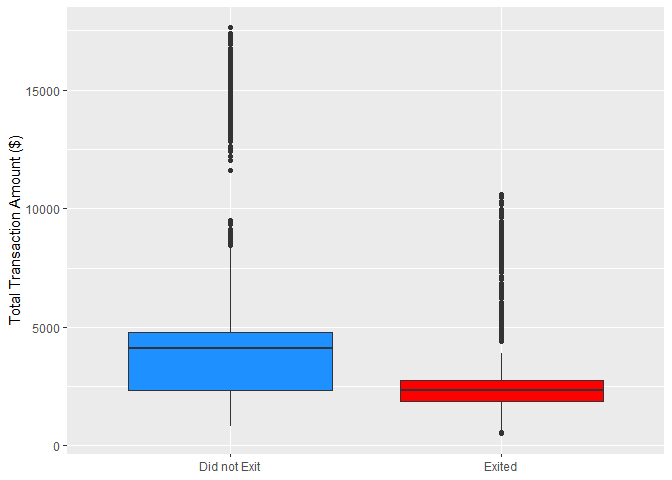
\includegraphics{Analysis_files/figure-latex/unnamed-chunk-30-1.pdf}

In Figure 31, the distributions of the total transaction counts are
shown in the form of boxplots for customers who exited the company and
who did not exit the company. Customers that exited the company
generally had significant fewer transactions with a median of about 40
compared to a median of about 70 for those who did not exit. The 75\%
percentile for the customers that exited is below the 25\% percentile
for the customers that did not exit, which demonstrates that transaction
count does a very good job at discriminating between if a customer exits
or not.

Figure 32
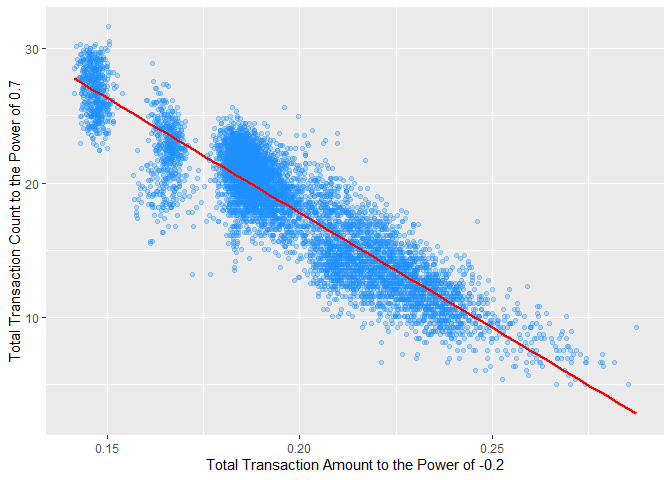
\includegraphics{Analysis_files/figure-latex/unnamed-chunk-31-1.pdf}

In Figure 32, distributions for the transaction amount in dollars
between the exited and did not exit customers demonstrates that
customers that exit generally spend less than customers that do not
exit. The third quartile for the exited group in terms of transaction
amount is only slightly above the first quartile of the did not exit
group. We can see that both groups generally spend about \$2,500 to
\$5,000 with their credit cards per year, but there are many outliers in
both groups.

The boxplots of the total transaction amounts overlap much more when
looking at the distribution of total transaction amount compared to
total transaction count, so tranaction count does a better job at
discriminating between exited or did not exit.

\textbf{Contingency Table}

Figure 33
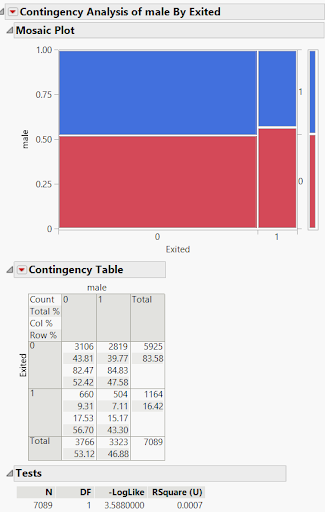
\includegraphics{https://github.com/hasiegler/STATProject/blob/main/LR1.png?raw=true}

The odds ratio from the contingency table Figure 33 is 1.18. This means
that female customers have 1.18 times the odds of exiting than males do.

Figure 34
\includegraphics{Analysis_files/figure-latex/unnamed-chunk-32-1.pdf}

The scatterplot in Figure 34 plots customers' transaction amount and
transaction counts and codes the points by if the customer exited or did
not exit. The scatterplot shows us that customers that exit generally
spent less and engage in fewer transactions than customers that did not
exit. Also, customers that exited the company almost never spent more
than \$10,000 in the year, however there are many customers that did not
exit that spend around \$15,0000.

\hypertarget{single-predictor-model}{%
\subsection{Single Predictor Model}\label{single-predictor-model}}

\textbf{Response Variable: Exit} \textbf{Explanatory Variable: Total
transaction count}

For this model we chose to use the total transaction count variable
because it appeared to discriminate between successes and failures
better based on the lack of overlap in the box plots compared to the box
plot for total amount spent.

From the estimates in Table 3.1, we will use the model to predict the
probability of a customer exiting given that the customer has a total
transaction count of 20 transactions.

\(\frac{e^{1.4038 - 0.05(20)}}{1 + e^{1.4038 - 0.05(20)}} = 0.58\)

0.58 means that a customer with 20 total transactions over the past year
has a predicted probability of exiting the company of 58\%. This is a
very high probability consider that only 16\% of all the customers in
the dataset exited the company. This suggests that people with lower
transaction counts are more likely to exit the company.

Figure 35
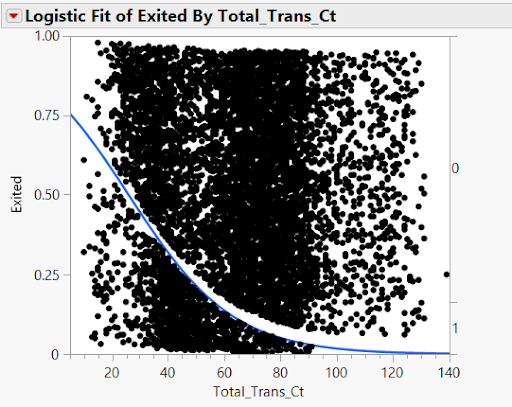
\includegraphics{https://github.com/hasiegler/STATProject/blob/main/LR3.png?raw=true}

Looking at the downward direction of the slope, we can tell that there
is a negative relationship between the total transaction count and the
probability that a customer will have exited the company. This is
evidenced by how the slope for the model is -0.0540, the negative
integer means that there is a negative relationship between likelihood
of a customer exiting and total transaction cost. The predicted
probability of a customer exiting for high transaction counts is very
close to zero, but the probability of customers exiting is not very
close to 1 for customers with low transaction counts.

To interpret the slope in the context of the model, for every
transaction that a customer makes, the odds of that customer exiting the
company decreases by \(e^{-0.05}\) times or 0.9474 times.

The computer's odds factor is 0.9474 in Table 3.2, with a 95\%
confidence interval of 0.943 to 0.9509. We are 95\% confident that the
true decrease in odds of exiting the company for an increase of 1 in
total transaction count is between 0.943 and 0.9509 times.

\(Ho: \beta_1 = 0\) The odds of exiting are the same for any level of
transaction count. \(Ha: \beta_1 \neq 0\) The odds of exiting are not
the same for different transaction counts.

The chisquared value associated with this test is 834, with a pvalue of
\textless.0001. Based on the small pvalue, we can reject the null
hypothesis and conclude that the total transaction count changes the
odds of a customer exiting. This test is consistent with the confidence
interval, because the confidence interval was all less than 1 for the
odds factor. If the odds factor included 1, it would mean that the odds
are not different for increases in transaction counts.

Figure 36
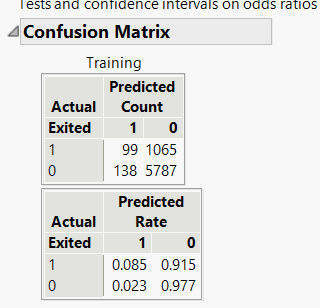
\includegraphics{https://github.com/hasiegler/STATProject/blob/main/LR5.png?raw=true}

The confusion matrix in Figure 36 lines up with our other data seeing as
it has high accuracy. The accuracy rate of .8303 or 83.03\%, means that
83.03\% of our predictions were correct. The model makes sense to use
because exit status did largely depend on tranaction count. Using only 1
predictor variable, an 83\% accuracy rate is fairly strong. Looking at
the scatterplot with transaction count by exit status, we can see that
as transaction count rise, the probability of exiting decreases for all
levels of transaction counts, so the model is appropriate. The only
unusual observations are the group of customers that have high total
transaction counts, but the model adequately accounts for the
probability of them exiting being very low.

\hypertarget{multiple-predictors-model}{%
\subsection{Multiple Predictors Model}\label{multiple-predictors-model}}

\(log(odds of exiting) = 1.03 - 0.43 Total\_Relationship\_Count - 0.0003 Total\_Trans\_Amt + 0.2male[0]\)

Using the model to predict the probability of a male customer with a
total relationship count of 6 and total transaction amount of \$920, we
can plug in the values into the following formula:

\(\frac{e^{1.033 - 0.43(6) - 0.0003(920) + 0.2049(0)}}{1 + e^{1.033 - 0.43(6) - 0.0003(920) + 0.2049(0)}} = 0.13\)

The predicted probability that an individual with these attributes exits
is 13\%.

From Table 3.3, based on the high ChiSquare value and low p-value of
\textless0.001 in the whole model test, we can conclude that the model
is a significant model in terms of whether or not a customer will exit
based on total translation amount, total relationship count, and gender.

In Table 3.4, based on the high ChiSquare values and low p-values for
all of our x variables, we can conclude that each variable is a
significant predictor for of the odds of a customer leaving the company.

\textbf{Drop in Deviance Test}

We will carry out a drop in deviances test for a full model with total
relationship count, total transaction amount, gender, and an interaction
between gender and total transaction amount. The reduced model has all
the same variables except for the interaction term.

\(D = 2(2848) - 2(2763) = 170\) Df = 4-3 = 1 and pvalue \textless.0001

After completing a drop in deviance test we can conclude that the full
model is better than the reduced model. The chi squared value is 170.26
with a small p value of \textless.0001. Since the interaction term is
significant, we acknowledge that odds of exiting based on total
transaction amount changes depending on gender.

\textbf{Residual Plot}

Figure 37
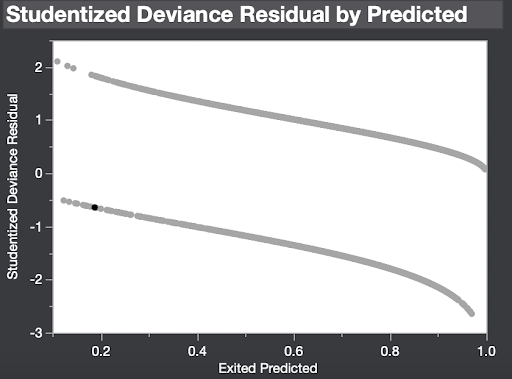
\includegraphics{https://github.com/hasiegler/STATProject/blob/main/LR8.png?raw=true}

There are a decent amount of points that have large residuals in Figure
37. There are only a few points with a large positive residual however,
there are more negative residuals.

Figure 38
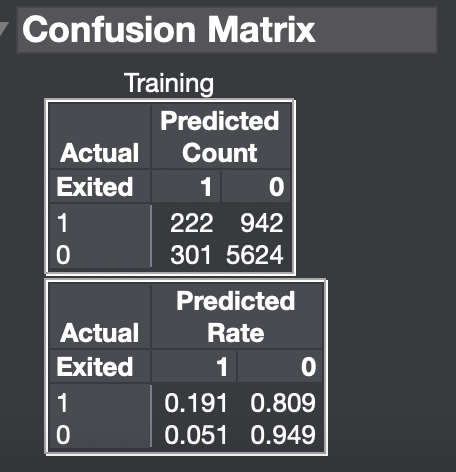
\includegraphics{https://github.com/hasiegler/STATProject/blob/main/LR9.png?raw=true}

Based on the confusion matrix in Figure 38, we have an accuracy rate of
82.46\%, which is actually a lower accuracy rate than in the single
predictor model, which was 83\%.

\hypertarget{conclusion-2}{%
\subsection{Conclusion}\label{conclusion-2}}

In the logistic regression section, we were interested in predicting the
probability that a customer exits the company, which is a binary
variable. We first used only transaction count to predict whether or not
a customer would exit. Then we used total relationship count, gender,
and total transaction amount as a predictor variables, but this model
actually had a lower accuracy rate than the single predictor model. I
would use the single predictor model, and add interaction terms and
other variables to that model to create the best accuracy for predicting
exit status.

\hypertarget{final-conclusion}{%
\section{Final Conclusion}\label{final-conclusion}}

In our report we examined a data set from a credit card company and
performed 3 different types of analysis, these included simple linear
regression, multiple regression, and logistic regression. For the first
analysis, we performed a simple linear regression where we sought to
predict the number of total transactions that a customer has had based
on the dollar amount that said customer spent using their credit card.
After plotting the initial data set, we found that all but the
independence assumption was violated, we aimed to correct this by
applying a number of transformations until we arrived at our final model
in which we decrease Y to the power of .7 and X to the power of -.02,
which provided us with a model that satisfied all out assumptions. This
model proved to be quite effective as it was a statistically significant
predictor of total transaction counts with a correlation of .8281, this
showed that there is a positive correlation between the amount a
customer spent and the number of transactions that the customer had.
This conclusion is along the lines of what we expected since it would
make sense a person who is spending large amounts of money is probably
making more transactions. One phenomenon that we witnessed was that the
customers with the largest negative residuals had almost all exited the
company.

The next analysis that we ran was a multiple regression model where we
sought to, like the simple linear regression model, predict the number
of total transactions that a customer would make, however, this time we
used multiple predictor variables. We transformed the total transaction
amount and total relationship count, and we used credit limit and exit
status. Overall, the final model is very strong and it predicts the
total transaction count of customers fairly accurately, with a typical
deviation of actual values from predicted values of 9, which is very
close considering the average transaction count is 65 transactions. The
overall model utility test suggests that our model is very significant
in predicting transaction count for these customers of this company. The
model is valid, as it generally satisfies all of the assumptions
required for multiple linear regression models. One weakness of the
model is that it is only a slight improvement in predicting transaction
count compared to the simple linear regression model with only
transaction amount transformed as a predictor variable. The R-squared
values for both models are similar, and our model is more complex due to
the extra terms that were added to the model. The final does tell us a
few things about the total transaction counts for customers. It tells us
customers that who have not exited generally have more transactions
compared to customers that exited, so if a customer is not engaging in
as many transactions, they are more likely to exit. Also, as the total
number of products held by a customer increases, the fewer transactions
the customer has on average, holding the other variables constant. Also,
we can see that increased transaction amounts are associated with higher
transaction counts, holding the other variables constant.

We also focused on predicting whether or not a customer would exit the
customer by running logistic regressions with the response variable
being 1 if the customer exits and 0 if the customer is still a current
customer. We found that the best predictor of exit status was total
transaction count, which had an accuracy rate of 83\%. The coefficient
was negative, which showed us that as the total transaction count
increases, the odds of a customer exiting decrease. Overall, there were
no unusually large residuals because the customers with large
transaction counts did not exit the company.

These three analyses gave us various insights into the habits of credit
card customers and how various attributes relate to each other. We saw
very distinct differences in spending depending on whether or not a
customer exited the company for example. We would have liked to have
more information on our dataset, such as how the customers were selected
to be placed in this dataset. We saw no customers that had extremely
large transaction amounts or counts, and the minimum transaction counts
and transaction amounts were capped. There were no customers with very
low transaction amounts, so there were definitely some criteria for how
customers were selected to be used in the dataset, of which we are
unaware. Finding out how and why certain customers were not included
would be ideal. Also, we did not look into detail the categorical
variables such as education status, income level, or the type of credit
card a customer has, which could have interesting results.

\hypertarget{appendix}{%
\section{Appendix}\label{appendix}}

Table 1.1

\begin{verbatim}
##                    Variable     N     Mean Std. Dev.    Min Pctl. 25 Pctl. 75
## 1              Customer_Age 10127   46.326     8.017     26       41       52
## 2           Dependent_count 10127    2.346     1.299      0        1        3
## 3            Months_on_book 10127   35.928     7.986     13       31       40
## 4  Total_Relationship_Count 10127    3.813     1.554      1        3        5
## 5    Months_Inactive_12_mon 10127    2.341     1.011      0        2        3
## 6     Contacts_Count_12_mon 10127    2.455     1.106      0        2        3
## 7              Credit_Limit 10127 8631.954  9088.777 1438.3     2555  11067.5
## 8       Total_Revolving_Bal 10127 1162.814   814.987      0      359     1784
## 9      Total_Amt_Chng_Q4_Q1 10127     0.76     0.219      0    0.631    0.859
## 10          Total_Trans_Amt 10127 4404.086  3397.129    510   2155.5     4741
## 11           Total_Trans_Ct 10127   64.859    23.473     10       45       81
## 12      Total_Ct_Chng_Q4_Q1 10127    0.712     0.238      0    0.582    0.818
## 13    Avg_Utilization_Ratio 10127    0.275     0.276      0    0.023    0.503
## 14                   Exited 10127    0.161     0.367      0        0        0
## 15                     male 10127    0.471     0.499      0        0        1
## 16                       id 10127     5064  2923.557      1   2532.5   7595.5
##      Max
## 1     73
## 2      5
## 3     56
## 4      6
## 5      6
## 6      6
## 7  34516
## 8   2517
## 9  3.397
## 10 18484
## 11   139
## 12 3.714
## 13 0.999
## 14     1
## 15     1
## 16 10127
\end{verbatim}

Table 1.3

\begin{verbatim}
##                          Total_Trans_Ct
## Exited                            -0.37
## Total_Relationship_Count          -0.24
## Contacts_Count_12_mon             -0.15
## Customer_Age                      -0.07
## male                              -0.07
## Months_on_book                    -0.05
## Months_Inactive_12_mon            -0.04
## Avg_Utilization_Ratio              0.00
## Total_Amt_Chng_Q4_Q1               0.01
## Dependent_count                    0.05
## Total_Revolving_Bal                0.06
## Credit_Limit                       0.08
## Total_Ct_Chng_Q4_Q1                0.11
## id                                 0.70
## Total_Trans_Amt                    0.81
## Total_Trans_Ct                     1.00
\end{verbatim}

Table 1.4

\begin{verbatim}
##          Variable     N     Mean Std. Dev. Min Pctl. 25 Pctl. 75   Max
## 1 Total_Trans_Amt 10127 4404.086  3397.129 510   2155.5     4741 18484
## 2  Total_Trans_Ct 10127   64.859    23.473  10       45       81   139
\end{verbatim}

Table 1.5
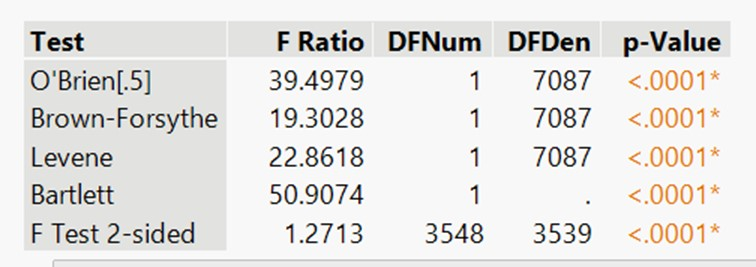
\includegraphics{https://github.com/hasiegler/STATProject/blob/main/SL2.jpg?raw=true}

Table 1.6
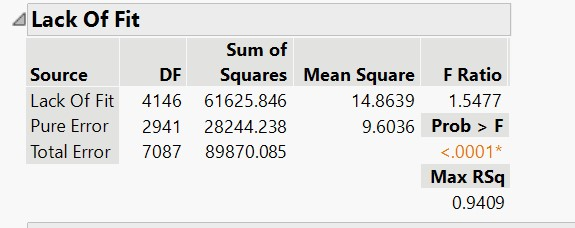
\includegraphics{https://github.com/hasiegler/STATProject/blob/main/SL1.jpg?raw=true}

Table 1.7
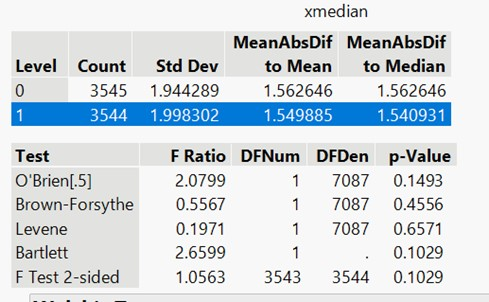
\includegraphics{https://github.com/hasiegler/STATProject/blob/main/SL3.jpg?raw=true}

Table 1.8
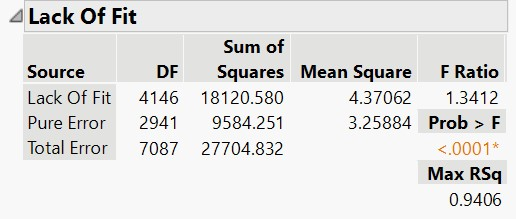
\includegraphics{https://github.com/hasiegler/STATProject/blob/main/SL4.jpg?raw=true}

Table 1.9
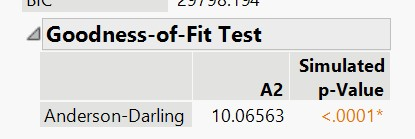
\includegraphics{https://github.com/hasiegler/STATProject/blob/main/SL5.jpg?raw=true}

Table 1.10
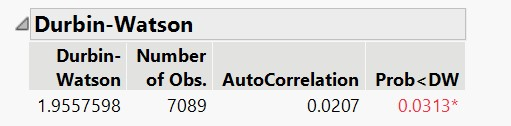
\includegraphics{https://github.com/hasiegler/STATProject/blob/main/SL7.jpg?raw=true}

Table 1.11

\begin{verbatim}
## # A tibble: 10 x 5
##    residual Exited Total_Trans_Amt Total_Trans_Ct Education_Level
##       <dbl>  <dbl>           <dbl>          <dbl> <chr>          
##  1    -9.30      1            6613             40 Uneducated     
##  2    -8.93      1            9177             50 High School    
##  3    -8.71      1            9183             51 High School    
##  4    -8.64      1            9061             51 Uneducated     
##  5    -8.52      1            5806             40 Graduate       
##  6    -7.60      1           10201             59 Uneducated     
##  7    -7.53      1            8325             54 Post-Graduate  
##  8    -7.50      0            1893             15 Graduate       
##  9    -7.48      1            8260             54 High School    
## 10    -7.44      1           10291             60 High School
\end{verbatim}

Table 1.12

\begin{verbatim}
## # A tibble: 5 x 5
##   residual Exited Total_Trans_Amt Total_Trans_Ct Education_Level
##      <dbl>  <dbl>           <dbl>          <dbl> <chr>          
## 1     7.59      0            2464             92 Uneducated     
## 2     7.25      0            1110             58 Doctorate      
## 3     7.21      0            3448            103 College        
## 4     7.10      0            3162             99 Graduate       
## 5     6.87      0            2465             88 Unknown
\end{verbatim}

Table 1.13

\begin{verbatim}
## # A tibble: 1 x 5
##   residual Exited Total_Trans_Amt Total_Trans_Ct Education_Level
##      <dbl>  <dbl>           <dbl>          <dbl> <chr>          
## 1     6.42      1             510             24 College
\end{verbatim}

Table 1.14

\begin{verbatim}
## 
## Call:
## lm(formula = I(Total_Trans_Ct^0.7) ~ I(Total_Trans_Amt^-0.2), 
##     data = training_data)
## 
## Residuals:
##     Min      1Q  Median      3Q     Max 
## -9.2956 -1.2705  0.1116  1.3894  7.5944 
## 
## Coefficients:
##                          Estimate Std. Error t value Pr(>|t|)    
## (Intercept)               51.9397     0.1839   282.4   <2e-16 ***
## I(Total_Trans_Amt^-0.2) -170.8788     0.9247  -184.8   <2e-16 ***
## ---
## Signif. codes:  0 '***' 0.001 '**' 0.01 '*' 0.05 '.' 0.1 ' ' 1
## 
## Residual standard error: 1.979 on 7087 degrees of freedom
## Multiple R-squared:  0.8281, Adjusted R-squared:  0.8281 
## F-statistic: 3.415e+04 on 1 and 7087 DF,  p-value: < 2.2e-16
\end{verbatim}

Table 1.15
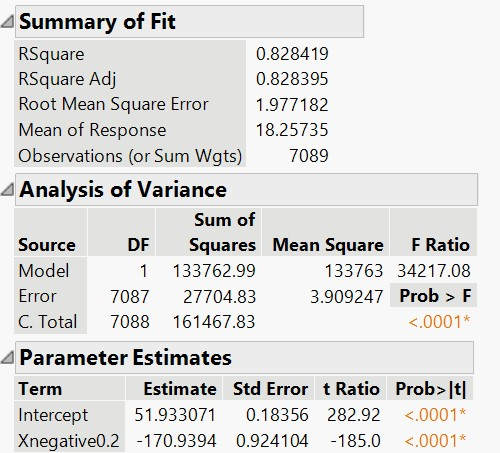
\includegraphics{https://github.com/hasiegler/STATProject/blob/main/SL10.jpg?raw=true}

Table 1.16
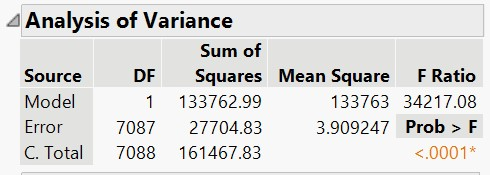
\includegraphics{https://github.com/hasiegler/STATProject/blob/main/SL11.jpg?raw=true}

Table 1.17

\begin{verbatim}
##        fit      lwr      upr
## 1 21.94403 21.88345 22.00462
\end{verbatim}

\begin{verbatim}
##        fit      lwr      upr
## 1 21.94403 18.06353 25.82453
\end{verbatim}

Table 1.18

\begin{verbatim}
## Correlation between testing data predictions and actual values 0.9109818
\end{verbatim}

Table 1.19

\begin{verbatim}
##                          Total_Trans_Ct Total_Trans_Amt      Exited
## Total_Trans_Ct               1.00000000       0.8070911 -0.37394933
## Total_Trans_Amt              0.80709113       1.0000000 -0.16994394
## Exited                      -0.37394933      -0.1699439  1.00000000
## Total_Relationship_Count    -0.23952972      -0.3508442 -0.14898082
## Credit_Limit                 0.07739854       0.1674287 -0.02450111
##                          Total_Relationship_Count Credit_Limit
## Total_Trans_Ct                        -0.23952972   0.07739854
## Total_Trans_Amt                       -0.35084421   0.16742873
## Exited                                -0.14898082  -0.02450111
## Total_Relationship_Count               1.00000000  -0.06403857
## Credit_Limit                          -0.06403857   1.00000000
\end{verbatim}

Table 2.1
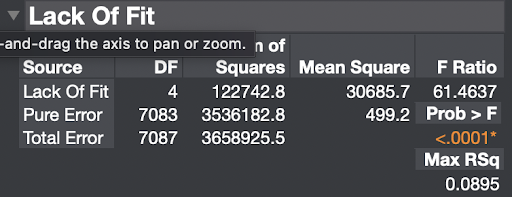
\includegraphics{https://github.com/hasiegler/STATProject/blob/main/ML5.png?raw=true}

Table 2.2
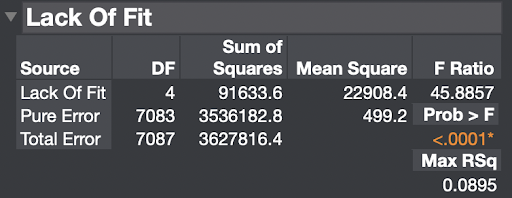
\includegraphics{https://github.com/hasiegler/STATProject/blob/main/ML6.png?raw=true}

Table 2.3
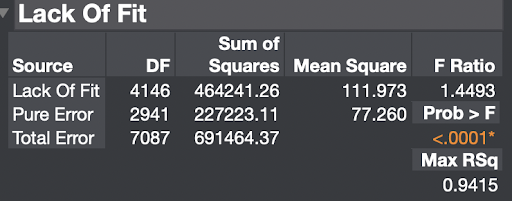
\includegraphics{https://github.com/hasiegler/STATProject/blob/main/ML8.png?raw=true}

Table 2.4
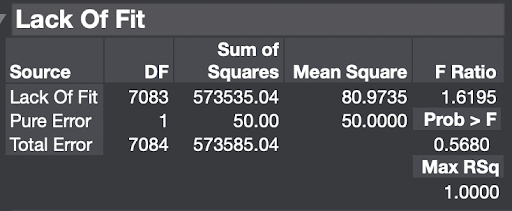
\includegraphics{https://github.com/hasiegler/STATProject/blob/main/ML10.png?raw=true}

Table 2.5
\includegraphics{https://github.com/hasiegler/STATProject/blob/main/ML11.png?raw=true}

Table 2.6
\includegraphics{https://github.com/hasiegler/STATProject/blob/main/ML14.png?raw=true}

Table 2.7
\includegraphics{https://github.com/hasiegler/STATProject/blob/main/ML15.png?raw=true}

Table 2.8
\includegraphics{https://github.com/hasiegler/STATProject/blob/main/ML16.png?raw=true}

Table 2.9
\includegraphics{https://github.com/hasiegler/STATProject/blob/main/ML17.png?raw=true}

Table 2.10
\includegraphics{https://github.com/hasiegler/STATProject/blob/main/ML18.png?raw=true}

Table 2.11
\includegraphics{https://github.com/hasiegler/STATProject/blob/main/ML19.png?raw=true}

Table 2.12

\begin{verbatim}
##        fit      lwr      upr
## 1 83.08467 82.78835 83.38098
\end{verbatim}

\begin{verbatim}
##        fit      lwr      upr
## 1 83.08467 65.42246 100.7469
\end{verbatim}

Table 2.13

\begin{verbatim}
## 
## Call:
## lm(formula = Total_Trans_Ct ~ Total_Trans_Amt + I(Total_Trans_Amt^2) + 
##     I(Total_Trans_Amt^3) + Marital_StatusDivorced + Marital_StatusMarried + 
##     Marital_StatusUnknown + Total_Relationship_Count + Exited, 
##     data = one_hot_training)
## 
## Residuals:
##     Min      1Q  Median      3Q     Max 
## -38.622  -6.098   0.053   5.845  40.044 
## 
## Coefficients:
##                            Estimate Std. Error t value Pr(>|t|)    
## (Intercept)               1.000e+01  6.370e-01  15.706  < 2e-16 ***
## Total_Trans_Amt           2.380e-02  2.998e-04  79.384  < 2e-16 ***
## I(Total_Trans_Amt^2)     -2.316e-06  4.932e-08 -46.968  < 2e-16 ***
## I(Total_Trans_Amt^3)      7.851e-11  2.145e-12  36.601  < 2e-16 ***
## Marital_StatusDivorced   -3.390e-01  4.240e-01  -0.800  0.42400    
## Marital_StatusMarried    -1.282e+00  2.331e-01  -5.500 3.94e-08 ***
## Marital_StatusUnknown    -1.353e+00  4.225e-01  -3.203  0.00137 ** 
## Total_Relationship_Count -2.308e-01  7.610e-02  -3.033  0.00243 ** 
## Exited                   -1.072e+01  3.093e-01 -34.653  < 2e-16 ***
## ---
## Signif. codes:  0 '***' 0.001 '**' 0.01 '*' 0.05 '.' 0.1 ' ' 1
## 
## Residual standard error: 8.9 on 7080 degrees of freedom
## Multiple R-squared:  0.8554, Adjusted R-squared:  0.8553 
## F-statistic:  5237 on 8 and 7080 DF,  p-value: < 2.2e-16
\end{verbatim}

Table 2.14

\begin{verbatim}
## Correlation between testing data predictions and actual values 0.9230898
\end{verbatim}

Table 2.15

\begin{verbatim}
## [1] 9.095798
\end{verbatim}

Table 3.1
\includegraphics{https://github.com/hasiegler/STATProject/blob/main/LR2.png?raw=true}

Table 3.2
\includegraphics{https://github.com/hasiegler/STATProject/blob/main/LR4.png?raw=true}

Table 3.3
\includegraphics{https://github.com/hasiegler/STATProject/blob/main/LR6.png?raw=true}

Table 3.4
\includegraphics{https://github.com/hasiegler/STATProject/blob/main/LR7.png?raw=true}

\end{document}
